	%%%%%%%%%%%%%%%%%%%%%%%%%%%%%%%%%%%%%%%%%%%%%%%%%%%%%%%%%%%%%%%%%%%%%%%%%%%
%%  esrel2022-paper.tex   :   19/12/2018 			                     %%
%%  Text file to use with rps-esrel2022. written in Latex2e.             %%
%%  The content, structure, format and layout of this style file is the  %%
%%  property of Research Publishing Services                             %%
%%  Copyright (c) 2011-2022 Research Publishing Services,                %%
%%  All rights are reserved.                                             %%
%%%%%%%%%%%%%%%%%%%%%%%%%%%%%%%%%%%%%%%%%%%%%%%%%%%%%%%%%%%%%%%%%%%%%%%%%%%

\documentclass[twocolumn]{rps-esrel2022}
%\documentclass[draft, twocolumn]{rps-esrl2012}

\def\papername{\jobname}

\def\ds{\displaystyle}


%\usepackage[authoryear]{biblatex-chicago}

\usepackage{natbib}
\usepackage{xcolor}
%\usepackage[marginparwidth=2.5cm]{geometry}
\usepackage[]{changes}
\usepackage{amsmath}
\usepackage{todonotes}
\usepackage{graphicx}
\usepackage{multicol}
\setcommentmarkup{\todo[color={authorcolor!20},size=\scriptsize]{#3: #1}}

\setlength{\marginparwidth}{2cm}

%% Rather hacky definition of an "annote"
%% by riding on \added
\newcommand{\note}[2][]{\added[#1,comment={#2}]{}}

\definechangesauthor[color=BrickRed]{AG}

\newcommand{\mda}[1]{\textcolor{blue}{#1}}

%\replaced[id=AG]{and the identification of parameters which require more empirical investment}

%\usepackage[authoryear]{natbib}

\begin{document}

\markboth{E. Miralles-Dolz, A. Gray, M. de Angelis, E. Patelli}{Interval-Based Global Sensitivity Analysis for Epistemic Uncertainty}

%%%%%%%%%%%%%%%%%%%%%%%%% Plase keep this command for single column for abstract section.
\twocolumn[
%%%%%%%%%%%%%%%%%%%%%%%%%

\title{Interval-Based Global Sensitivity Analysis for Epistemic Uncertainty}

\author{Enrique Miralles-Dolz}

\address{Institute for Risk and Uncertainty, University of Liverpool, United Kingdom. \email{enmidol@liverpool.ac.uk}}
\address{Culham Centre for Fusion Energy, United Kingdom Atomic Energy Authority, United Kingdom}

\author{Ander Gray}

\address{Institute for Risk and Uncertainty, University of Liverpool, United Kingdom. \email{akgray@liverpool.ac.uk}}
\address{Culham Centre for Fusion Energy, United Kingdom Atomic Energy Authority, United Kingdom}

\author{Marco de Angelis}

\address{Institute for Risk and Uncertainty, University of Liverpool, United Kingdom. \email{mda@liverpool.ac.uk}}

\author{Edoardo Patelli}

\address{Centre for Intelligent Infrastructure, University of Strathclyde, United Kingdom. \email{edoardo.patelli@strath.ac.uk}}

\begin{abstract}
     The objective of sensitivity analysis is to understand how the input uncertainty of a mathematical model contributes to its output uncertainty.
	In the context of a digital twin, sensitivity analysis is of paramount importance for the automatic verification and validation of physical models, and the identification of parameters which require more empirical investment. Yet, sensitivity analysis often requires making
	assumptions, e.g., about the probability distribution functions of the input factors, about the model itself, or relies on surrogate models for the evaluation of the sensitivity that also introduce more assumptions. %It can be the case that one cannot reliably assign probability distribution functions if the model is dominated by epistemic uncertainties, or the complexity of the model is such that surrogate models cannot accurately capture its behaviour.

	We present a non-probabilistic sensitivity analysis method which requires no assumptions about the input probability distributions: the uncertainty in the input is expressed in the form of intervals, and employs the width of the output interval as the only measure. %The method also returns all the information that could be obtained with the reduction of the input interval to a single value, i.e. pinching. 
	We use the Ishigami function as test case to show the performance of the proposed method, and compare it with Sobol' indices.
\end{abstract}

\keywords{ uncertainty quantification, sensitivity analysis, interval arithmetic, sobol indices, digital twin.}

%%%%%%%%%%%%%%%%%%%%%%%%% Please keep this closing bracket to complete the single column format for abstract.
]
%%%%%%%%%%%%%%%%%%%%%%%%%

\section{Introduction}
% Prediction
Prediction is inherent to science since it is essential to test theories and their consequences.
%Thanks to the power of modern computation, the prediction of natural phenomena represented by mathematical models can now be tested at unprecedented scales.
With modern digital computing, the prediction of natural phenomena represented by mathematical models can now be tested at unprecedented scales.

This digital transformation has led to the emergence of digital twins, which attempt to improve the predictive capability of the models using data.
"The aspiration of a digital twin is a close one-to-one mapping between a physical and virtual system", quoting \cite{wagg2020digital}; which brings enormous challenges, including that of dealing with model verification and validation.
The verification of such computational models without reliance on subjectivity is therefore of paramount importance (\cite{JRC122132}).
%\mda{This digital transformation has led to the emergence of digital twins, which improve predictive capability by augmenting computational simulation models using data.}
%The main transformative aspect of the digital twin is to improve predictive capability by augmenting computational models using data; this again reflects the wider digital transformations happening in society. 
% Digital twins exploit this advantage by modelling physical systems and allowing their evaluation via simulation, as these systems are often technically and
% economically prohibitive to operate in the physical world (\cite{wagg2020digital}).
%However, digital twins are often so complex that it is not possible to infer their prediction from experience and judgement alone.
%\mda{``The aspiration of a digital twin is a close one-to-one mapping between a physical and virtual system'' quoting  \citep{wagg2020digital}; which brings enormous challenges, including that of dealing with code complexity.
%The verification of such computational model without subjectivity is thus paramount (\cite{JRC122132}).}
%Therefore, it is desirable to verify and validate the prediction of these models without having to rely on subjectivity (\cite{JRC122132}).
%not sure to cite The Value of Using Imprecise Probabilities in Engineering Design here
Sensitivity analysis can help with this task, by indicating what model parameters are responsible for the prediction of the model, and how that prediction depends on them (\cite{saltelli2004sensitivity}).

According to \cite{razavi2021future}, sensitivity analysis methods can be classified in three main approaches: derivative-based, distribution-based, and regression-based, while other approaches (such as variogram-based) are generally a combination of these.
Derivative-based approaches compute the derivative of the model functions, either analytically or numerically, and measure the change in
the output when the inputs are perturbed around a base point (e.g., see \cite{errico1997adjoint}).
Distribution-based methods, such as Sobol' indices, decompose the output variance and assigns the partitions to the input variances, indicating how much
of the output variance is caused by each input variance alone or in combination with other inputs (\cite{saltelli2010variance}).
Lastly, regression-based approaches employ correlation coefficients, regression coefficients, or other machine learning methods (\cite{sudret2008global}).

However, these approaches present some limitations.
For instance, the analytical descriptions of the functions in the model are not always available, since it is not uncommon to deal with black-box models or
models with too many functions that make their analytical derivation unpractical or difficult.
Also, derivative-based methods require defining a base point for each input parameter, and a perturbation size.
It is not rare to find a situation without consensus about these elements.
A similar argument can be made for distribution-based methods, which require a precise definition of the probability distributions of model inputs.
Regression-based methods require a degree of knowledge of the behavior of the model under investigation, which is not always known.
For example, partial correlation coefficients assume model linearity, or monotonicity in the case of partial rank coefficients (\cite{saltelli1990non}).
%maybe add GP and PCE criticism
For these reasons, it is desirable to find a sensitivity analysis method that is independent on the model behaviour and requires limited knowledge of input parameters or no additional arbitrary assumptions.
%
%\begin{itemlist}
%
%	\item{}  Does not require knowing the analytical description of the model functions.
%	\item{}  Does not require defining base values for any input parameter.
%	\item{}  Does not require to assume that the input parameters follow a precise probability distribution function.
%	\item{}  Does not depend on the model behavior.
%
%\end{itemlist}
%
This paper presents an interval-based global sensitivity analysis method that fulfills these requirements.
%mention that 2,3,4 are related to epistemic uncertainty?
%Section 2 introduces some basic concepts in interval uncertainty propagation which are required to perform the analysis.
%In Section 3 it is explained how the sensitivity indices are calculated in the interval approach, and the
%pinching measure that can be calculated additionally.
%Lastly, Section 4 compares the performance of the interval-based method against Sobol' indices in two test cases for the
%Ishigami function, followed by a discussion and the conclusion in sections 5 and 6 respectively.

%\begin{enumerate}
%	\item Explain sensitivity analysis. [DONE]
%	\item Explain main approaches and their limitation. [DONE]
%	\item Explain epistemic uncertainty in engineering -slides- (we cannot afford those limitations) [DONE]
%	\item Explain structure of the paper [DONE]
%\end{enumerate}

\section{Interval Analysis}

With interval analysis it is possible to determine the bounds of the output of a function and capture its imprecision. Expressing parameter uncertainties in the form of intervals has the advantage of requiring no assumptions about the uncertainty other than its existence between two bounds, making intervals suitable for modelling epistemic uncertainty.

Interval arithmetic and sampling are the main methods to compute with intervals.
In the former, the mathematical operations are replaced to account for intervals as in \cite{moore2009introduction}.
This method requires access to the analytical description of the models (i.e. source code) to make them suitable for
interval arithmetic.
Sampling methods, on the other hand, do not require to adapt the source code for interval arithmetic.
A typical sampling procedure begins assuming uniform distributions for the uncertain parameters, performing
the sampling using e.g. the Latin Hypercube algorithm, and extracting the minimum and maximum of the outputs of interest 
(e.g., see \cite{helton2010representation}).
The main drawback of sampling methods is that the resulting output interval will be an inner approximation instead of an outer approximation (a desirable feature in safety assessments). However, sampling based sensitivity indices can be obtained at not extra cost from the samples used for uncertainty quantification as shown in \cite{PLISCHKE2013536} or from inference analysis in Credal Network as in \cite{Tolo2018126} .

The sensitivity analysis presented in this paper can be applied with both methods of interval analysis, employing the widths of the input and output intervals as
the only required measures.
Therefore, it can be used with black-box or sophisticated models that cannot be adapted to work with interval arithmetic (and therefore the uncertainty propagation
has to be performed via sampling), or with models which already adopt interval arithmetic.

%\begin{enumerate}
%	\item Explain epistemic uncertainty can be modeled as intervals. [DONE]
%	\item Explain interval uncertainty can be propagated with: arithmetic, sampling [DONE]
%	\item In te case the analytical function(s) are available, interval arithmetic gets the rigorous calculation.
%	If the function(s) are not available, the propagation can be performed with sampling. [DONE]
%\end{enumerate}

\section{Interval-Based Sensitivity Index}

The proposed sensitivity index captures the dependence of the model output on the inputs measuring the area described by these.
Figure 1 serves as an illustrative example.
It shows the scatterplots of the evaluation of a black-box function $y = f(x_1,x_2)$ with $x_1,x_2 \in [-5,5]$, with samples generated using Latin Hypercube sampling.
As explained in \cite{helton2003latin}, scatterplot visualisation is a straightforward qualitative method of inspecting dependencies in a model.
In this example it is possible to see how $y$ has a linear-like dependence with $x_1$ (Figure 1 (a)), but shows little or no dependence with $x_2$ (Figure 1 (b)).
The objective is to turn this qualitative \textit{intuition} into a measurement.

\begin{figure}[!b]
	\centering
	\begin{tabular}{@{}c@{}}
	  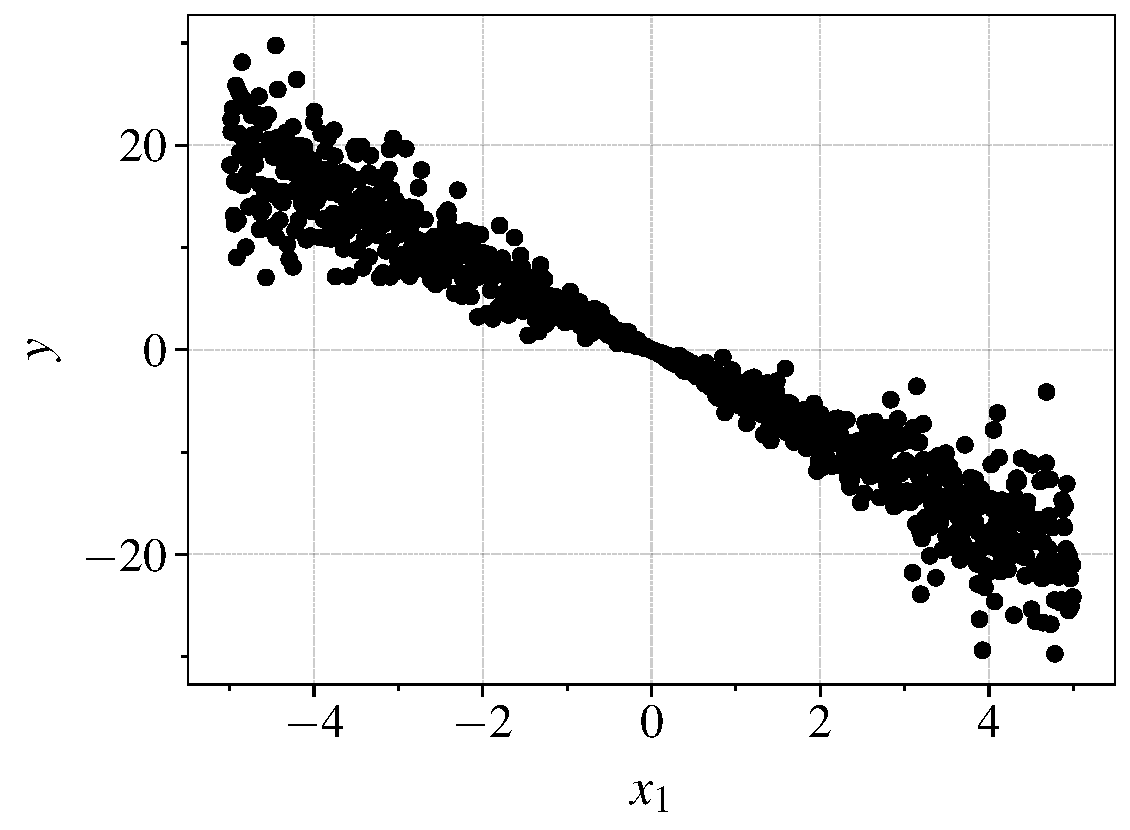
\includegraphics[width=0.94\linewidth]{figures/example_x1_grid.pdf} \\
	  \small (a) Scatterplot of $y=f(x_1,x_2)$ and $x_1$.
	\end{tabular}

	\begin{tabular}{@{}c@{}}
	  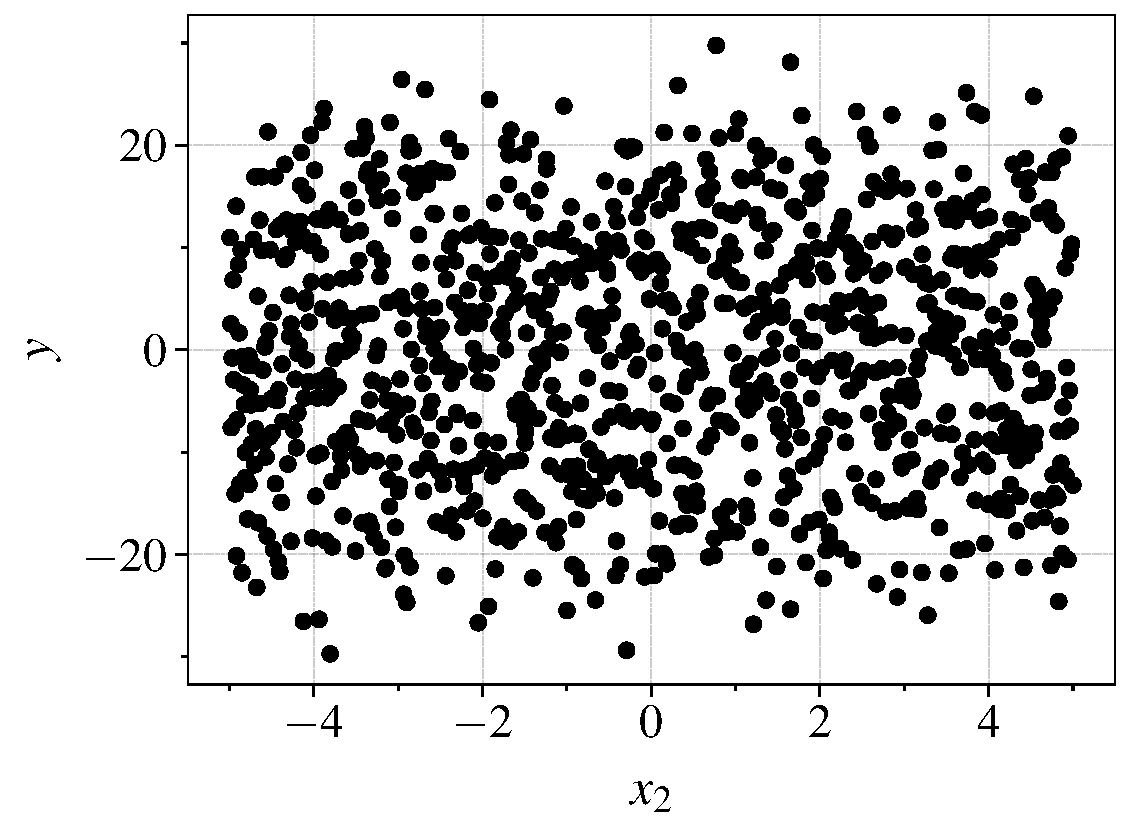
\includegraphics[width=0.94\linewidth]{figures/example_x2_grid.pdf} \\
	  \small (b) Scatterplot of $y=f(x_1,x_2)$ and $x_2$.
	\end{tabular}

	\caption{Results of the evaluation of a black-box function $y=f(x_1,x_2)$ with $x_1,x_2 \in [-5,-5]$ using 1000 samples generated with Latin Hypercube sampling.}
	%Function $y$ shows strong dependence with $x_1$, but little or no dependence with $x_2$.}
	\label{fig:myfig}
\end{figure}

The dependence can be captured measuring the area described by the scatterplot, and comparing it with the box defined by $[\underline{y},\overline{y}]\times[\underline{x_i},\overline{x_i}]$, where $\underline{y},\overline{y}$ are the minimum and maximum of $y$, and $\underline{x_i},\overline{x_i}$ the minimum and maximum of the $i^{\text{th}}$ input parameter.
If the measured area equals to the box area, the output has little or no dependence on that input;
if the measured area has a value of 0, the output is determined by that input. Any other degree of dependence will fall in-between these two extreme cases.

The sensitivity index is calculated with the following formula:
%
\begin{equation}
	S_i = 1 - \frac{\sum_n^N(\underline{x_i},\overline{x_i})_n\times(\underline{y},\overline{y})_n}{(\underline{y},\overline{y})\times(\underline{x_i},\overline{x_i})}{,}
\label{eq1}
\end{equation}
%
\noindent where $N$ is the total number of subintervals.
Therefore, $S_i$ is a sensitivity index ranging from 0 (i.e. $y$ cannot be determined from $x_i$) to 1 (i.e. $y$ is exactly determined by $x_i$).
Note that the measurement of the output area is an approximation of the actual area, being a consequence of the two different methods employed to solve the model functions: sampling method or subintervalisation.
The approximation can be improved increasing the number of samples or subintervals, to the detriment of computational cost.

The area can be calculated with two different methods depending on whether interval arithmetic was employed to calculate the function uncertainty or it was done through sampling. 
In the case of interval arithmetic the calculation is straightforward as the subintervals can be recycled and the rectangles described by these can be computed \textit{for free}.
If sampling methods were used, the area can be calculated binning the samples, finding the minimum $\underline{y}$ and maximum $\overline{y}$ in each bin, and calculating the area of each bin.
The main drawback of the sampling method is that a step size has to be defined for the binning, and the impact of this parameter on the proposed sensitivity analysis method has not been studied yet.
%employing an integration method similar to the Riemann sum: a step size is defined to sweep through subintervals of $x_i$ in the data, the minimum $\underline{y}$ and maximum $\overline{y}$ are retrieved for each subinterval, and the rectangle area is computed as usual.
%However, since the method is similar to the Riemann sum, it may be possible to place error bounds on the accuracy of the sensitivity index. 

Figure \ref{fig:myfig1} shows the areas calculated with the sampling approach.
The algorithm requires the output and input data, and the number of subintervals to divide it. In this example 20 subintervals were used.
Then the minimum and maximum output are found for each subinterval, and the area of the rectangle is calculated.
The total measured area defined by the scatterplot is then the sum of all the rectangles' areas.

\begin{figure}[!b]
	\centering
	\begin{tabular}{@{}c@{}}
	  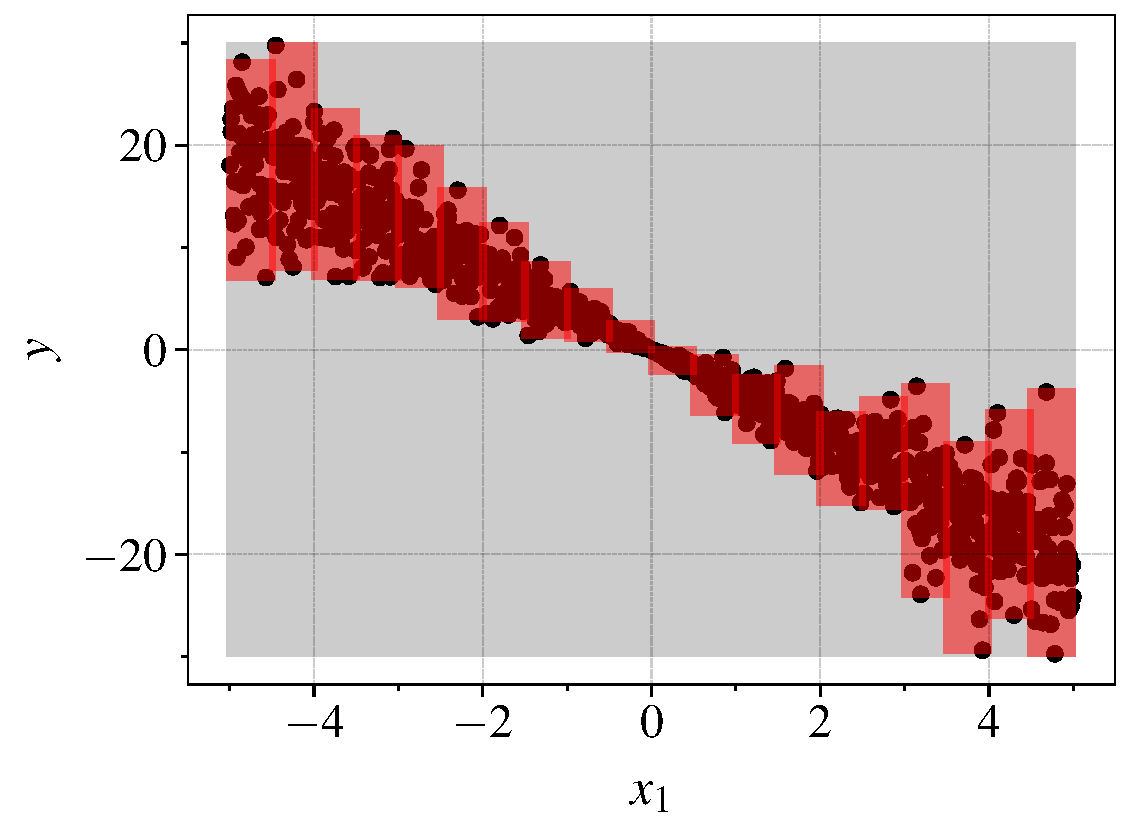
\includegraphics[width=0.94\linewidth]{figures/example_sampling_x1_grid.pdf} \\
	  \small (a) Measured scatterplot area (red) and box area (grey)\\
	  \small of $y=f(x_1,x_2)$ and $x_1$.
	\end{tabular}

	\begin{tabular}{@{}c@{}}
	  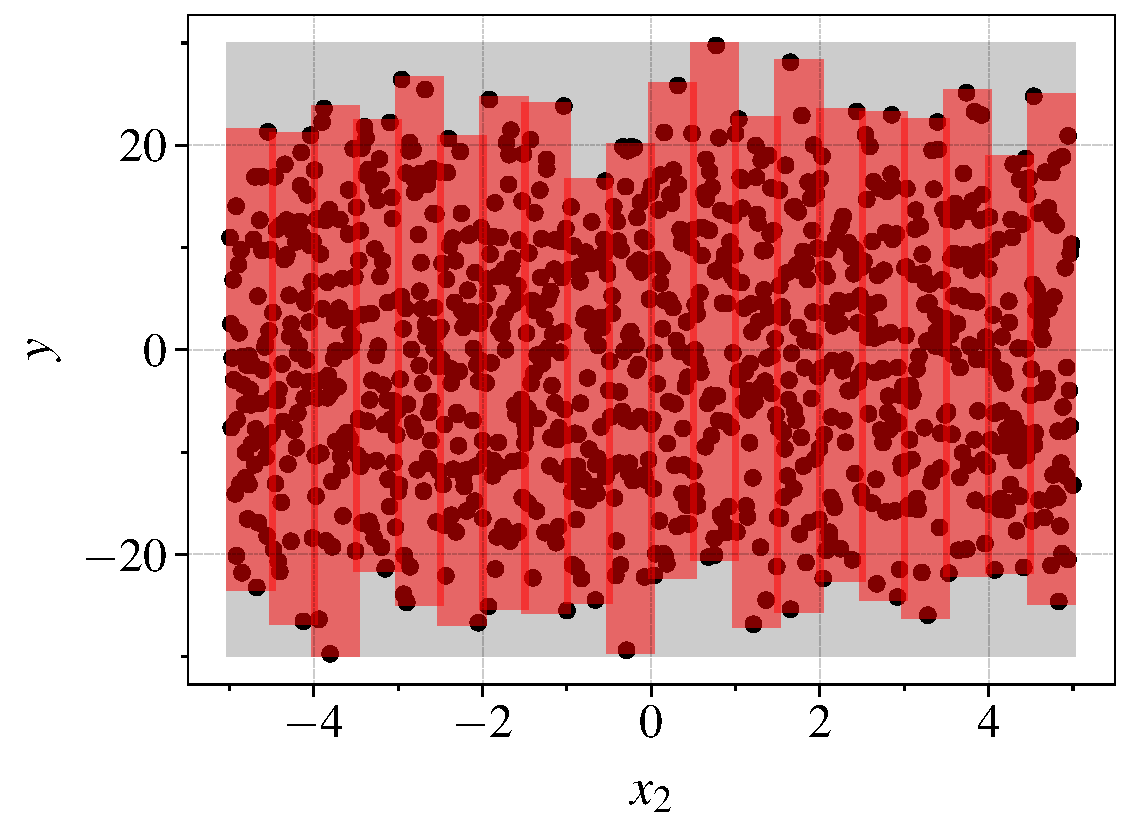
\includegraphics[width=0.94\linewidth]{figures/example_sampling_x2_grid.pdf} \\
	  \small (b) Measured scatterplot area (red) and box area (grey)\\
	  \small of $y=f(x_1,x_2)$ and $x_2$.
	\end{tabular}

	\caption{Results of the evaluation of $y=f(x_1,x_2)$ with $x_1,x_2 \in [-5,-5]$ using 1000 samples generated with Latin Hypercube and 20 subintervals.
	The sensitivity index is calculated as in Eq. \ref{eq1}, where the numerator is equal to the area coloured in red and the denominator
	equal to the area coloured in grey.}
	%Function $y$ shows strong dependence with $x_1$, but little or no dependence with $x_2$.}
	\label{fig:myfig1}
\end{figure}

Figure 3 shows the 20 subintervals computed with interval arithmetic using the IntervalArithmetic.jl Julia package (\cite{benet2020juliaintervals}).
Note that since the function $y = f(x_1,x_2)$ is a black-box function, access to its analytical form is restricted, and therefore the interval arithmetic approach would not be possible. However, it has been included as an example to show how the interval arithmetic approach would work.

The sensitivity indices for $x_1,x_2$ calculated with the sampling and arithmetic approaches are displayed in Table 1.
Both approaches return the same ordering, indicating that $x_1$ is the dominant parameter.
Note that the interval arithmetic approach captures that $x_2$ has no impact on the uncertainty of $y$ (it can  also be seen in Figure \ref{fig:width}(b), since the
red area equals to the grey area, making $S_2 = 0$), whilst the sampling approach is not as precise.
This is caused by the fact that the sampling approach is an inner approximation method, and the greater the number of samples, the more accurate the sensitivity index is.

\begin{table}[!h]
	\tbl{Interval-based sensitivity indices for $x_1$ ($S_1$) and for $x_2$ ($S_2$).}
	{\tabcolsep14pt
	\begin{tabular}{@{}lll@{}}\toprule 
	Sensitivity Index  & Sampling  & Interval arithmetic\\
\colrule

	$S_1$ & 0.790 & 0.732\\
	$S_2$ & 0.197 & $\approx 0$\\
\botrule
	\end{tabular}}

\end{table}

\begin{figure}[!b]
	\centering
	\begin{tabular}{@{}c@{}}
	  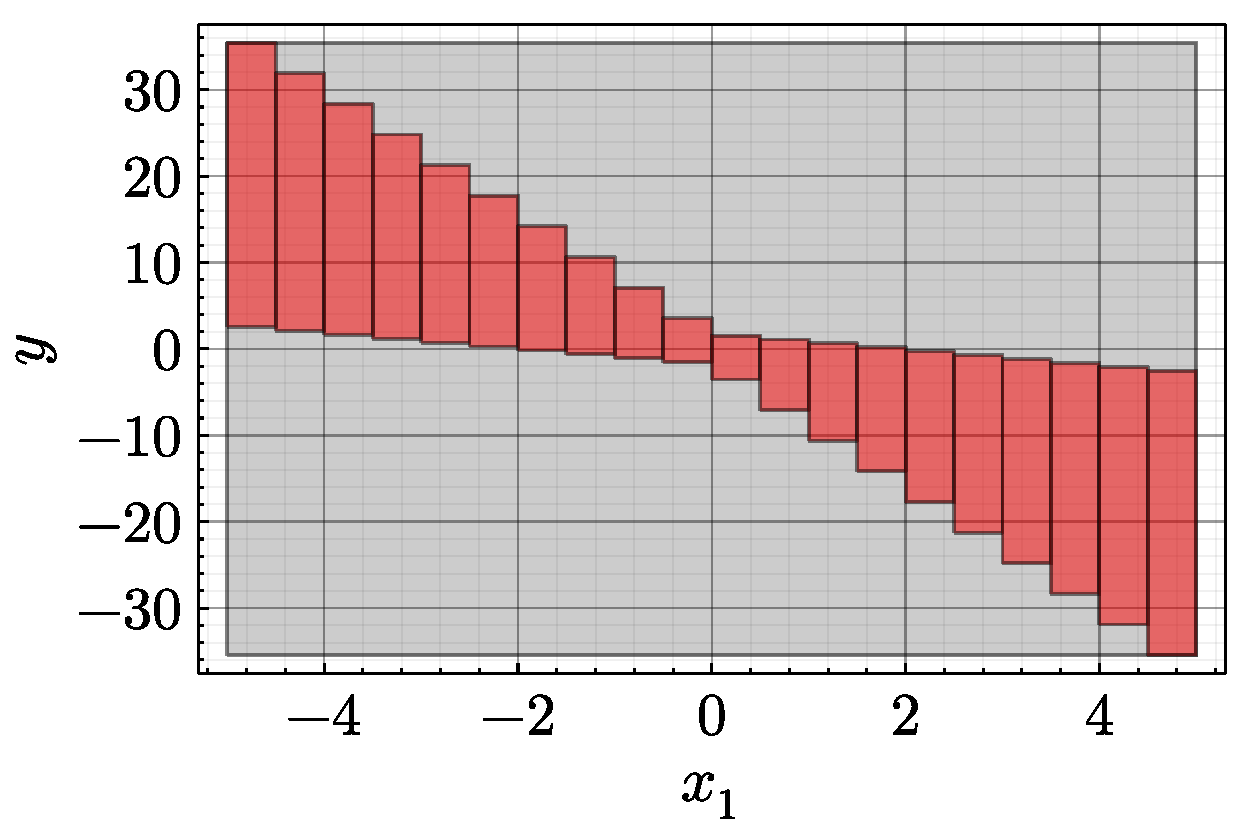
\includegraphics[width=0.94\linewidth]{figures/example_boxes_1.pdf} \\
	  \small (a) Visualisation of the 20 subintervals\\
	  \small of $y=f(x_1,x_2)$ and $x_1$.
	\end{tabular}

	\begin{tabular}{@{}c@{}}
	  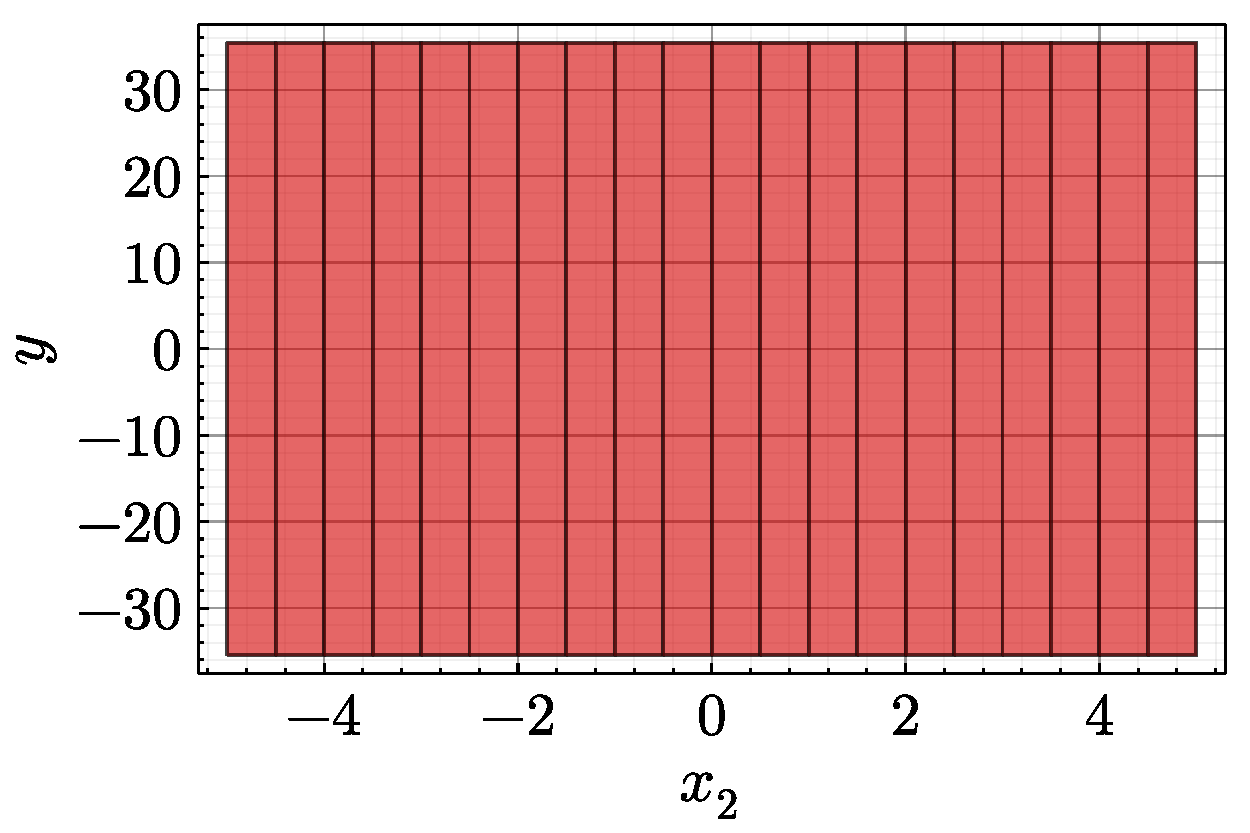
\includegraphics[width=0.94\linewidth]{figures/example_boxes_2.pdf} \\
	  \small (b) Visualisation of the 20 subintervals\\
	  \small of $y=f(x_1,x_2)$ and $x_2$.
	\end{tabular}

	\caption{Results of the evaluation of $y=f(x_1,x_2)$ with $x_1,x_2 \in [-5,-5]$ using 20 subintervals and interval arithmetic.
	The sensitivity index is calculated as in Eq. \ref{eq1}, where the numerator is equal to the area coloured in red and the denominator
	equal to the area coloured in grey.}
	%Function $y$ shows strong dependence with $x_1$, but little or no dependence with $x_2$.}
	\label{fig:myfig}
\end{figure}

Lastly, an important by-product of the proposed sensitivity index is that its calculation also entails the so called \textit{pinching} method.
The \textit{pinching} sensitivity analysis calculates the reduction on the output uncertainty when the uncertainty of an input is reduced from the interval to a single value (e.g., see \cite{ferson2006sensitivity,PatelliUQ, gray2022inference}).
One drawback of this method is that a single value for each input interval has to be chosen (or several values within the interval, with the consequent
increase of computational cost).
However, the interval-based sensitivity index retrieves all the \textit{pinching} information possible for the given number of subintervals; so not only the
output dependence on the input is measured, but also how the input affects the output across its domain.
Figure \ref{fig:width} shows how reducing uncertainty in $x_2$ entails no reduction on the uncertainty of $y$, whilst reducing the uncertainty on $x_1$ has different consequences on the
uncertainty of $y$ depending on the value of $x_1$.
For example, the best uncertainty reduction is obtained pinching at $x_1 = 0$.

\begin{figure}[!t]
    \label{fig:width}
	\centering
	\begin{tabular}{@{}c@{}}
	  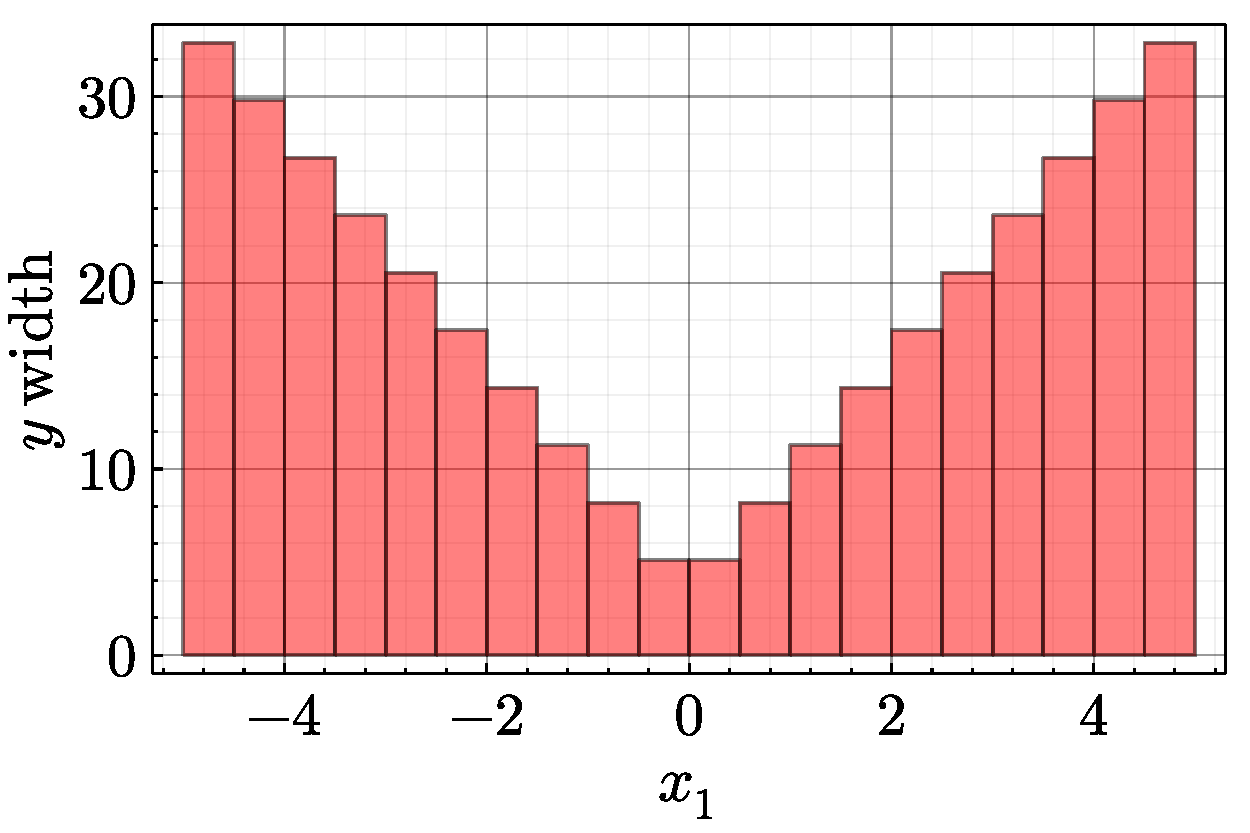
\includegraphics[width=0.94\linewidth]{figures/example_pinching_1.pdf} \\
	  \small (a) Output width of $y$ across $x_1$.
	\end{tabular}

	\begin{tabular}{@{}c@{}}
	  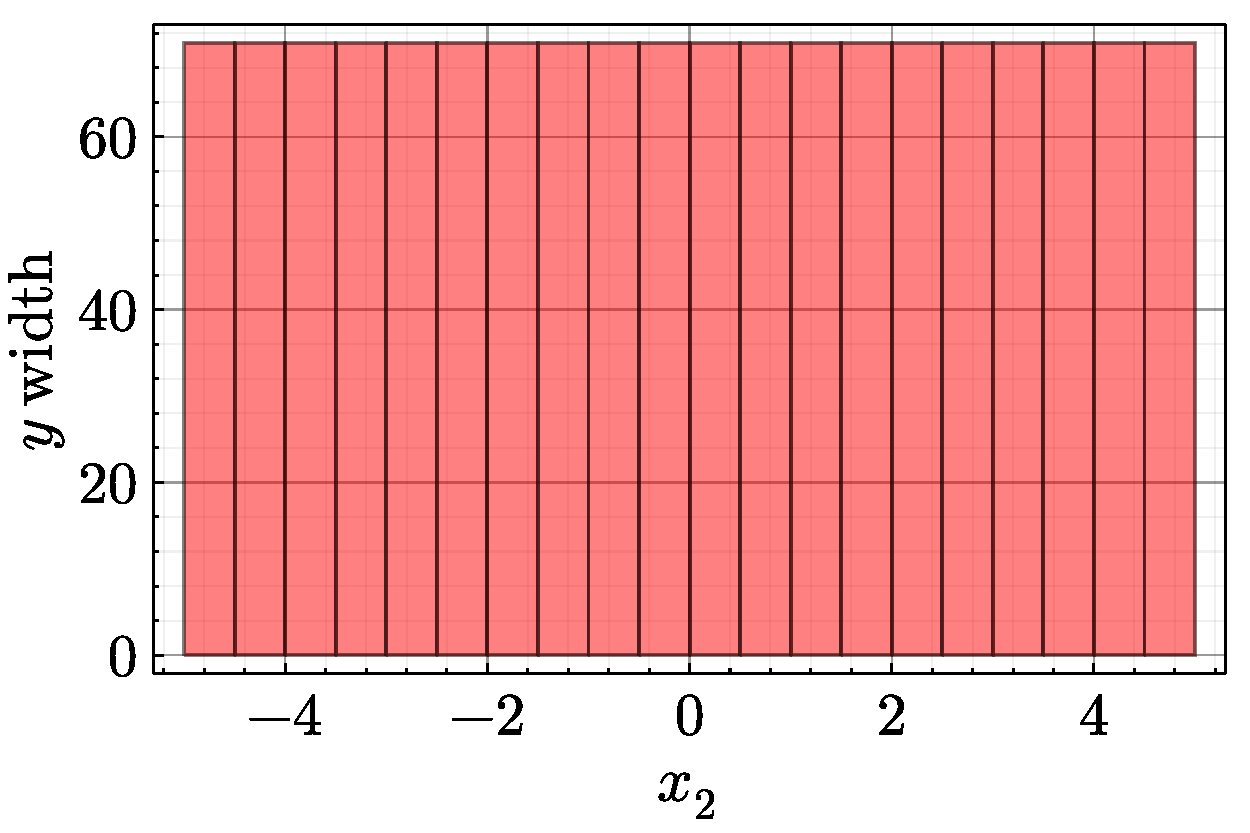
\includegraphics[width=0.94\linewidth]{figures/example_pinching_2.pdf} \\
	  \small (a) Output width of $y$ across $x_2$.
	\end{tabular}

	\caption{Output width of $y=f(x_1,x_2)$ across the domain of $x_1$ and $x_2$. This method
	calculates the output uncertainty when reducing the input parameter uncertainty to a subinterval or
	point value.}

\end{figure}

%\begin{enumerate}
%	\item Introduce the area method (overview and illustrating example). [DONE]
%	\item Use example and extreme cases to illustrate (e.g. perfect dependence = index of 1 = no area, independence = index of 0 = all area) [DONE]
%	\item Show equation of the sensitivity index [DONE]
%	\item Explain how it does with arithmetic (subintervalisation) [DONE]
%	\item Explain how it does with sampling (integration similar to trapezoid rule) [DONE]
%	\item Explain pinching. [DONE]
%\end{enumerate}

\section{Application}

To show the performance of the proposed interval-based global sensitivity analysis method, we compare
its results in terms of parameter ranking with the Sobol' indices on the Ishigami function, which is a common benchmark in the uncertainty quantification and sensitivity analysis community for its non-linearity, non-monotonicity, and the interaction effects between $x_1$ and $x_3$ (\cite{ishigami1990importance}). The Ishigami function is
%
    \begin{multline}
	f(x_1,x_2,x_3) =  \\  \sin(x_1) + a\sin^2(x_2) + b\sin(x_1)x_3^4{,}
	\end{multline}
%
\noindent where the constants are set to $a=5$ and $b=0.1$, and the input variables $x_1,x_2,x_3$ are in $[-\pi,\pi]$.
%
Since the analytical formula of the function is known, the interval-based sensitivity analysis can be performed with interval
arithmetic.
Figure 5 shows the results of the interval analysis of the Ishigami function with 100 subintervals for $x_1$, $x_2$, and $x_3$, with their corresponding sensitivity
indices indicated in Table 2, calculated following the methodology presented in Section 3.
According to the interval-based method, the Ishigami function has the highest dependence with $x_3$, followed by $x_1$.

\begin{figure}[!t]
	\centering
	\begin{tabular}{@{}c@{}}
	  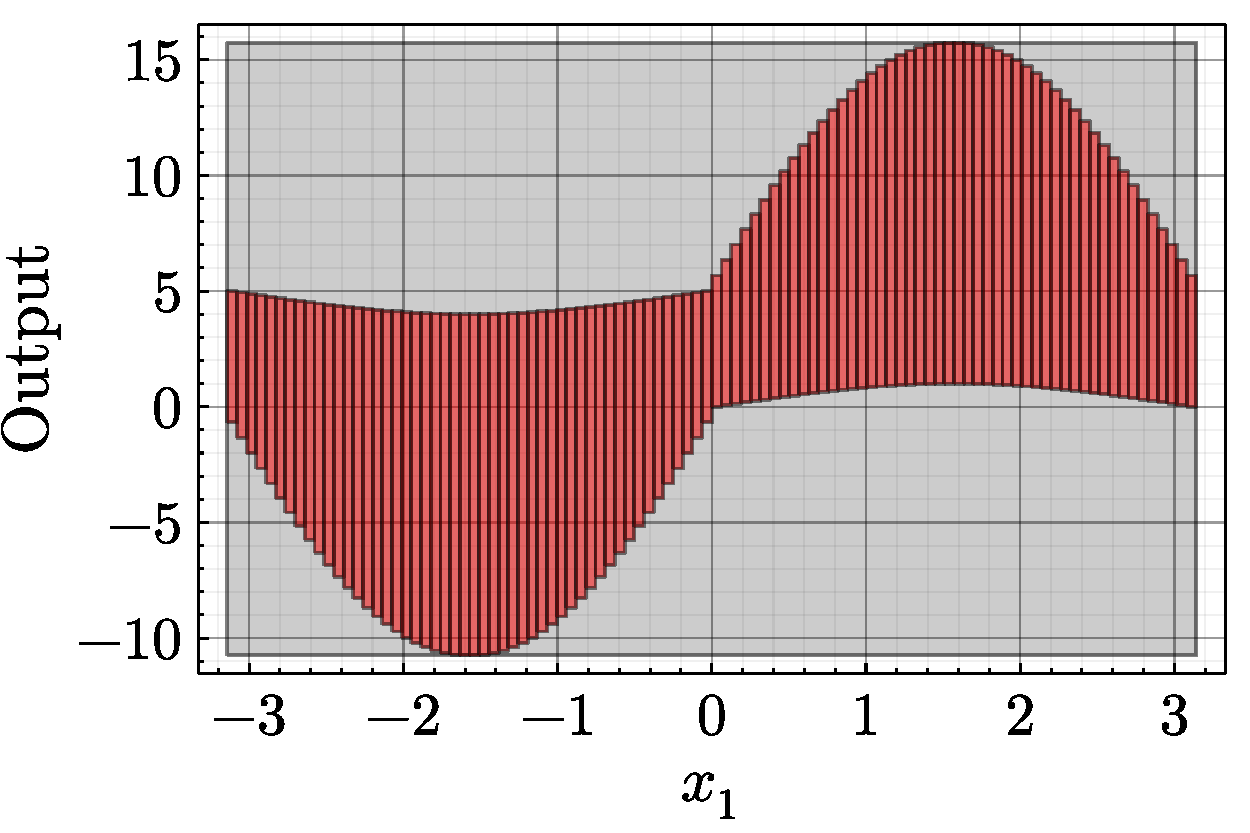
\includegraphics[width=0.94\linewidth]{figures/ishigami_1.pdf} \\
	  \small (a) Intervalisation of the Ishigami function\\
	  \small and $x_1$ using 100 subintervals.
	\end{tabular}

	\begin{tabular}{@{}c@{}}
	  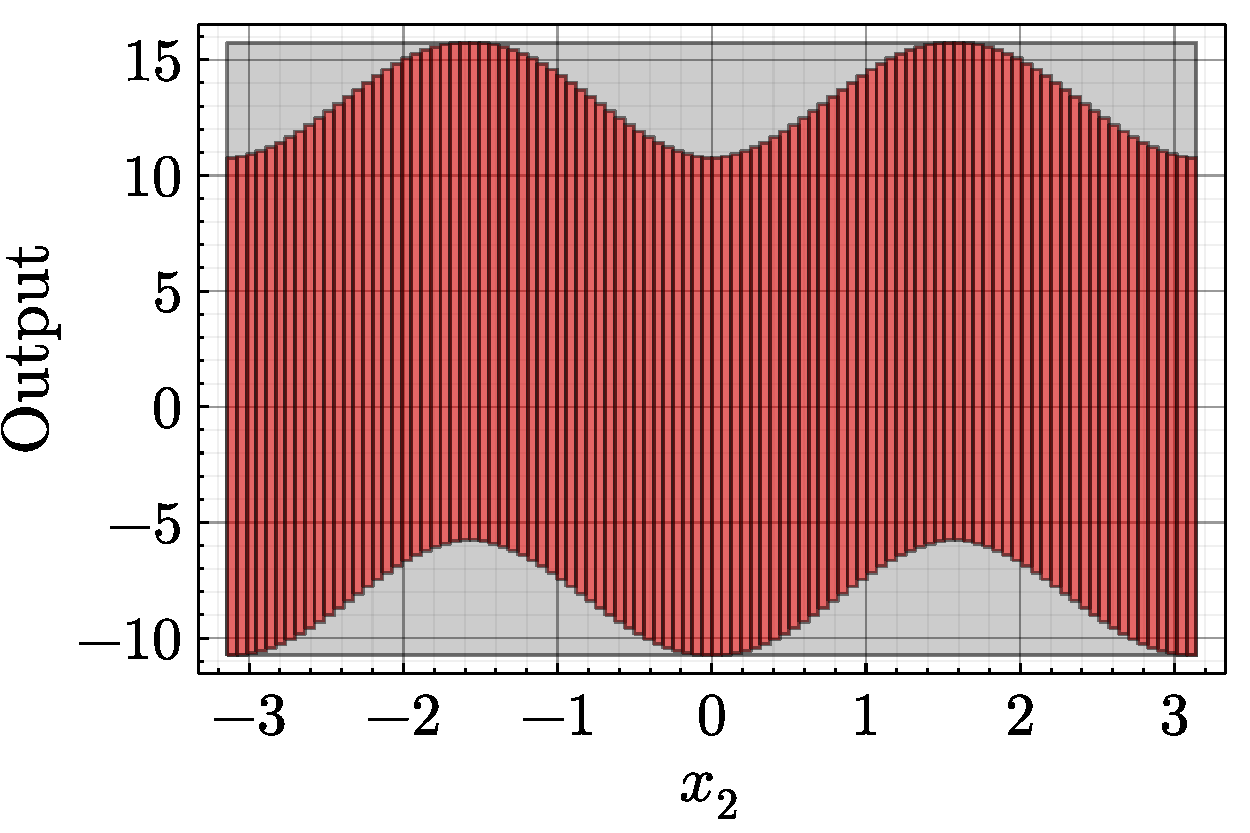
\includegraphics[width=0.94\linewidth]{figures/ishigami_2.pdf} \\
	  \small (b) Intervalisation of the Ishigami function\\
	  \small and $x_2$ using 100 subintervals.
	\end{tabular}

	\begin{tabular}{@{}c@{}}
		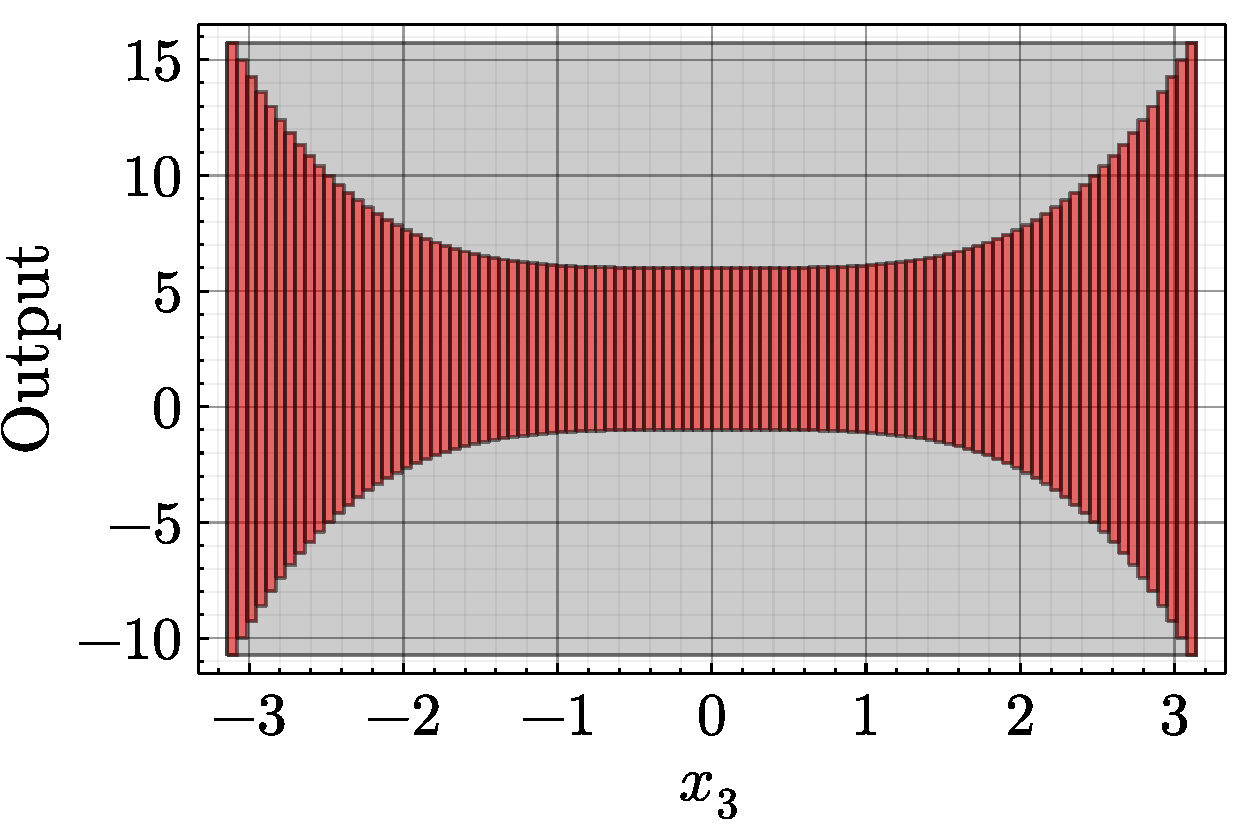
\includegraphics[width=0.94\linewidth]{figures/ishigami_3.pdf} \\
		\small (c) Intervalisation of the Ishigami function\\
		\small and $x_3$ using 100 subintervals.
	  \end{tabular}

	\caption{Results of the evaluation of the Ishigami function with $x_1,x_2,x_3 \in [-\pi,\pi]$ with interval arithmetic using 100 subintervals.
	}
\end{figure}

%In addition to the sensitivity indices, the interval-based approach also provides all the information of the \textit{pinching} analysis.
Figure 6 shows the uncertainty on the Ishigami output when pinching $x_1$, $x_2$, and $x_3$.
The maximum reduction on the Ishigami uncertainty is achieved when $x_1$ is fixed to $-\pi$, $0$, or $\pi$.
If pinching any of the three parameters to a point value were not possible, the second best strategy to maximise the output uncertainty
reduction would be to pinch the $x_3$ interval from $[-\pi,\pi]$ to $[-1,1]$, as Figure 6(c) suggests.
Lastly, pinching $x_2$ entails almost the same uncertainty reduction, and the smallest of the three parameters, across its entire domain.

\begin{figure}[!t]
	\centering
	\begin{tabular}{@{}c@{}}
	  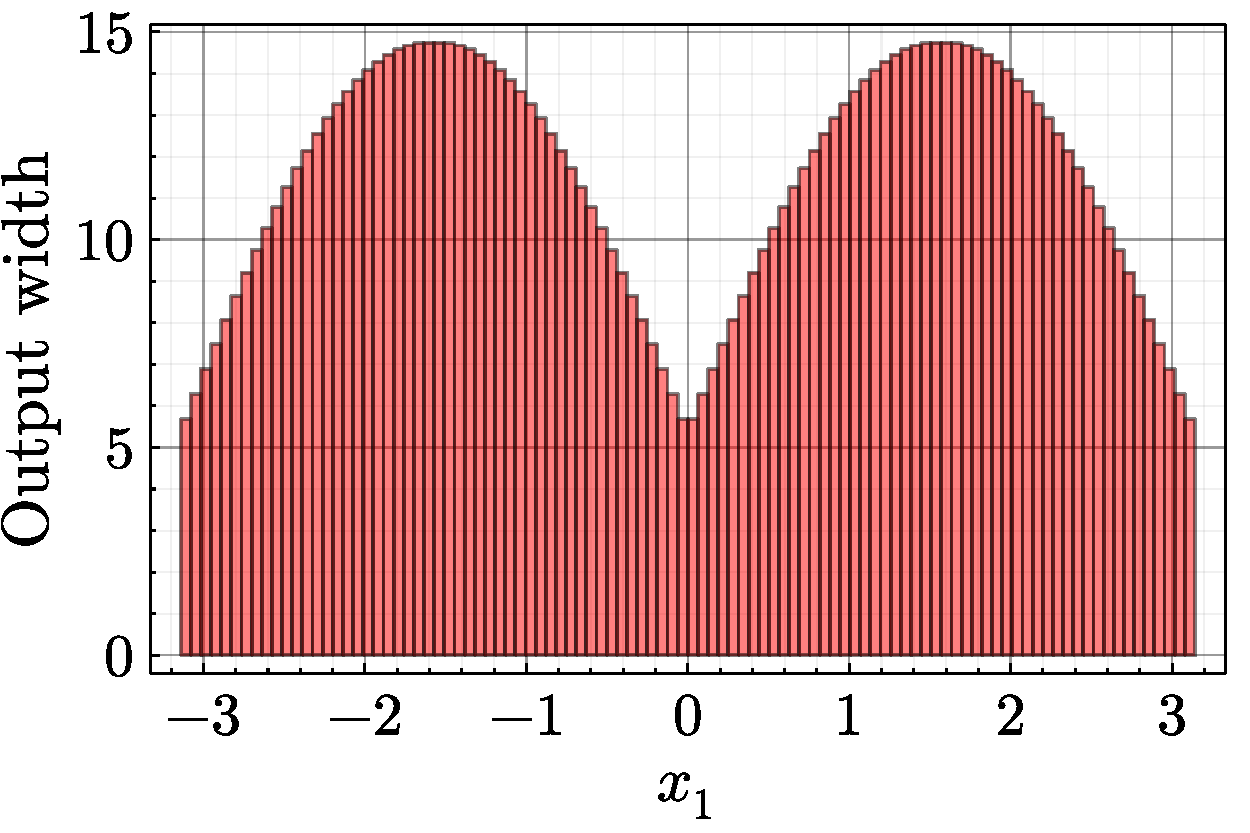
\includegraphics[width=0.94\linewidth]{applications/ishigami_pinching_1.pdf} \\
	  \small (a) Output width of the Ishigami function\\
	  \small across $x_1$.
	\end{tabular}

	\begin{tabular}{@{}c@{}}
	  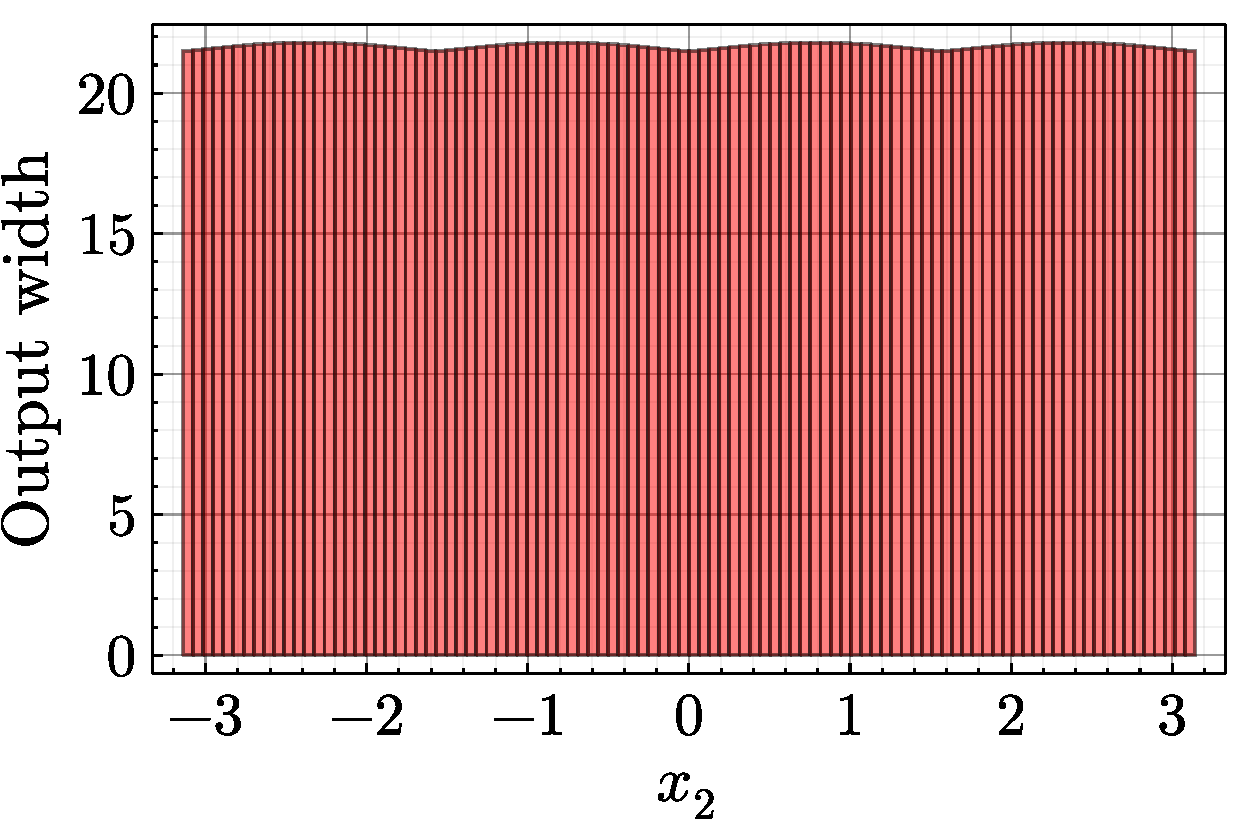
\includegraphics[width=0.94\linewidth]{applications/ishigami_pinching_2.pdf} \\
	  \small (b) Output width of the Ishigami function\\
	  \small across $x_2$.
	\end{tabular}

	\begin{tabular}{@{}c@{}}
		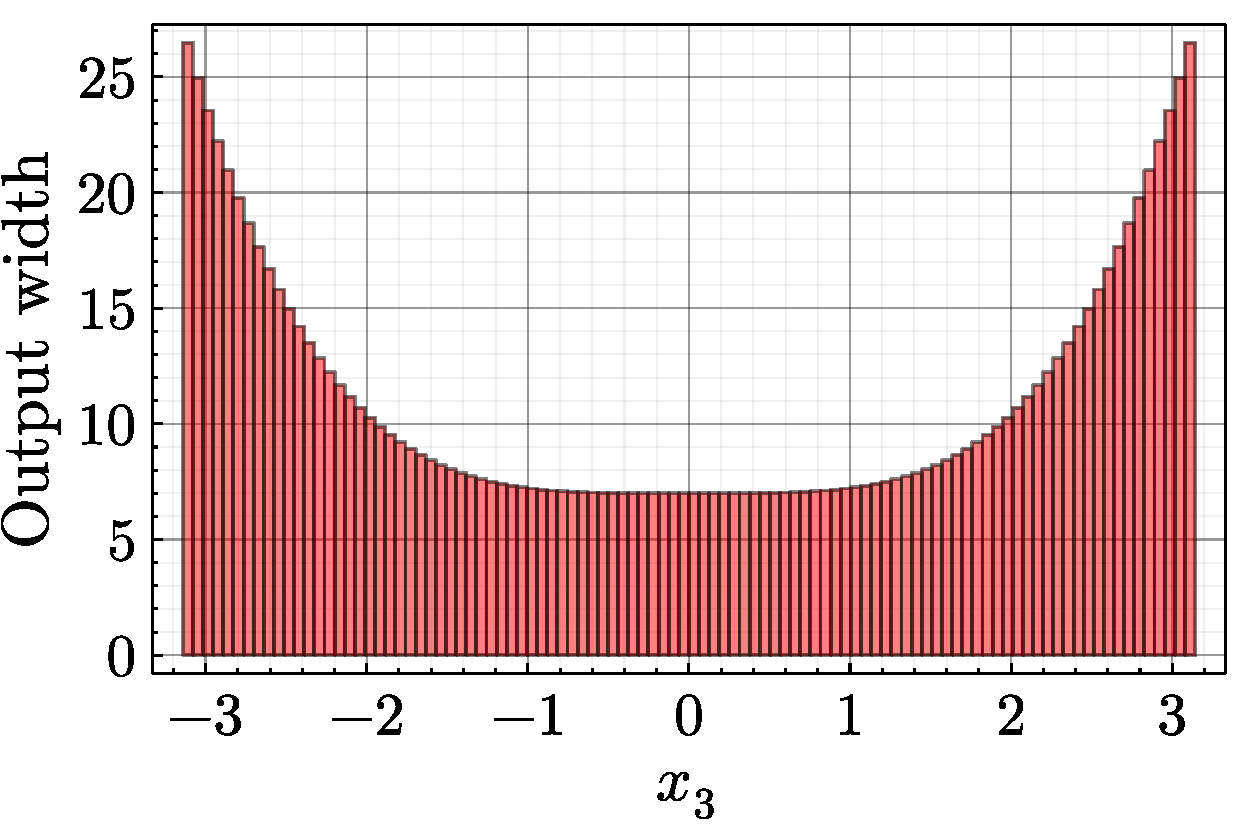
\includegraphics[width=0.94\linewidth]{applications/ishigami_pinching_3.pdf} \\
		\small (c) Output width of the Ishigami function\\
		\small across $x_3$.
	  \end{tabular}

	\caption{Output width of the Ishigami function across the domain of $x_1$, $x_2$, and $x_3$.
	}
\end{figure}

\begin{table*}[!h]
	\tbl{Interval-based and Sobol' sensitivity indices of the Ishigami function. The interval arithmetic based indices were calculated with 100 subintervals. The Sobol' indices for the uniform case were calculated analytically while  for the triangular case were calculated with 2048 samples generated with Saltelli sampling.}
	{\tabcolsep14pt
	\begin{tabular}{@{}llllll@{}}\toprule 
	 &  & \multicolumn{2}{c}{Uniform distribution} & \multicolumn{2}{c}{Triangular distribution} \\ \colrule
	 Sensitivity Index & \multicolumn{1}{c|}{Interval-based} & First Order & \multicolumn{1}{c|}{Total} & First Order & Total \\ \colrule

	$S_1$ & 0.568 & 0.400 & 0.711 & 0.254 & 0.409\\
	$S_2$ & 0.181 & 0.288 & 0.288 & 0.591 & 0.591\\
	$S_3$ & 0.581 & $\approx 0$ & 0.311 & $\approx 0$ & 0.158\\
\botrule
	\end{tabular}}
\end{table*}

When the inputs of the Ishigami function are independent and uniformly distributed in $[-\pi,\pi]$, the analytical description of the variance
terms used to calculate the Sobol' indices are known; therefore the exact first order and total Sobol' indices can be calculated in this case.
Table 2 contains the analytical Sobol' indices of the Ishigami function.
Analytically, the variance of $x_1$ is the greatest contributor to the variance of the Ishigami function, and $x_3$ has effect on the Ishigami
only when interacting with $x_1$.

A second case for the Ishigami function has been included where the input variables follow a triangular distribution in $[-\pi,\pi]$ with mode in $0$. This example is used to support the issue when the distribution functions of the input variables are not totally known, showing
that the Sobol' indices could be sensible to these assumptions.
To calculate the Sobol' indices for the triangular case, 2048 samples were generated using the Saltelli sampling method, which is an extension of the Sobol'
sequence optimised for calculating the indices (\cite{saltelli2002making}).
Table 2 shows the results of the analysis.
The results suggest that, in this case, the variance of $x_2$ is the greatest contributor to the variance of the Ishigami.
Note that the uncertainties on the indices have been omitted since these were negligible, and had no impact on the final parameter ranking.

%\begin{enumerate}
%	\item Explain Ishigami function [DONE]
%	\item Perform IBGSA [DONE]
%	\item Perform Sobol with uniforms[DONE]
%	\item Perform Sobol with triangular [DONE]
%	\item Show pinching. [DONE]
%\end{enumerate}

\section{Discussion}

When the inputs of the Ishigami function are expressed as intervals, without assuming any distribution function,
the interval-based sensitivity analysis claims that $x_3$ is the most important parameter, since the Ishigami function
shows the highest dependence on it, followed by $x_1$.
Sobol' indices were employed in two different cases of the Ishigami function: one with inputs following an uniform distribution in $[-\pi,\pi]$, and another with inputs were assumed to follow a triangular distribution
in $[-\pi,\pi]$ with mode at $0$.
In the uniform case, $x_1$ was the first ranked parameter. In the triangular case, $x_2$ was the first ranked parameter.
These results highlight the fact that variance-based methods for sensitivity analysis can return contradictory results when the input distribution function is not accurately known and the variance may not be a reliable statistic.

Furthermore, in the context of digital twins it is important not only to perform parameter prioritisation to find on which parameter to focus the uncertainty reduction, but also to find the most effective reduction in output uncertainty.
The results from the interval-based approach suggest that, if reducing input uncertainty to a point value were possible, pinching
$x_1$ to $-\pi$, $0$, or $\pi$ would entail the optimum output uncertainty reduction.
If reducing to a point value were too restrictive (technically, economically...), reducing the uncertainty of $x_3$ from $[-\pi,\pi]$
to $[-1,1]$ would be the best option.
Generally, in variance-based methods the output uncertainty reduction is an average reduction of its variance when the variance of certain input
is reduced some \% (e.g., see \cite{allaire2012variance}).
In that regard, intervals may be easier to interpret than variances, and therefore the interval-based approach could offer an advantage.

Variance-based methods provide information about interaction effects in the model (as it does with $x_1$ and $x_3$),
and this is a feature that has not been explored with the interval-based approach.
This feature is definitely useful for model diagnostic, and therefore Sobol' indices can be a useful complement to the
interval-based approach.
Generally, it is desirable to include as many sensitivity analysis methods as possible, as these answer to different questions
and can help to better understand the problem under investigation.

%\begin{enumerate}
%	\item Explain results of interval
%	\item discuss what happens with sobol (variance based)
%	\item compare methods (Sobol says which to reduce but does not say how to reduce)
%	\item One could argue both methods are answering two different questions (dependence vs variance), which is true.
%	The objective of this paper is to introduce a sensitivity analysis method with minimum amount of assumptions and reiterate
%	that variance-based methods could return misleading results when the variance is not a reliable statistic.
%	This is the case of scenarios under epistemic uncertainty.
%\end{enumerate}
%Sobol good for interaction effects, IB lacks
%Factor priorisation in terms of variance reduction is a bit confusing.
%When designing stuff it is much straightforward to work with intervals rather than variances.
%"For factor priorisation purposes then, the conclusion that is drawn from the analysis is to focus future research efforts
%on factor x1, since on average once fixed, factor x1 is expected to reduce the variance of Y by the largest amount".
%weird.

\section{Conclusion}

This paper introduces an interval-based method for performing global sensitivity analysis with interval analysis, computed either
via sampling method or with interval arithmetic.
This method only requires expressing the input parameter uncertainty in the form of intervals, and therefore is particularly
suited for cases under epistemic uncertainty.
Also, calculating the interval-based sensitivity indices also retrieves all the information of the pinching method,
which measures the output uncertainty reduction when input uncertainty is reduced to a point value or subinterval.

The interval-based approach was applied on the Ishigami function, and its results were compared with the Sobol' indices. The results presented have shown the importance of the  knowledge about the probability distribution function of the inputs (i.e. epistemic uncertainty), when variance based methods are used for sensitivity analysis.  
This effect was illustrated using uniform and triangular distribution functions for the inputs of the Ishigami where the Sobol' indices returned contradictory results when the input distributions were changed.
In this respect, when the inputs are not precisely known the interval-based approach is more reliable since it returns the same parameter ranking for a given input domain.
This is an initial work towards sensitivity analysis methods for epistemic uncertainty, and further work should be done to better understand the nature and limitations of the metric presented in this paper.

The code and algorithms used for the production of this document are available in the following repository: \url{https://github.com/Institute-for-Risk-and-Uncertainty/interval-sensitivity}

%\begin{enumerate}
%	\item Brief recap (we show a SA method blabla..) [DONE]
%	\item Method for epistemic uncertainty (no assumptions) [DONE]
%	\item This method can be used with interval arithmetic or sampling (blackbox) [DONE]
%	\item Compare its performance with Sobol on the Ishigami (sobol good for interaction) [DONE]
%	\item Further work [DONE]
%\end{enumerate}

\begin{acknowledgement}
This research was funded by the EPSRC and ESRC CDT in Risk and Uncertainty (EP/L015927/1), established within the Institute for Risk and Uncertainty at the University of Liverpool.
This work has been carried out within the framework of the EUROfusion Consortium, funded by the European Union via the Euratom Research and Training Programme (Grant Agreement No 101052200 — EUROfusion). Views and opinions expressed are however those of the author(s) only and do not necessarily reflect those of the European Union or the European Commission. Neither the European Union nor the European Commission can be held responsible for them.
\bibliographystyle{chicago}
\bibliography{References}
\end{acknowledgement}


\end{document}




